\section{Implementation Issues and Performance Estimation}
\label{sec:issues}

The performance of a TC is commonly related to ~\cite{biblio:tc_perf}, ~\cite{biblio:tc_perf_2
following features: 

\begin{itemize}
    \item Timestamps accuracy 
    \item Correction factor stability
    \item Maximum update rate
    \item Rapid reconfiguration after topology changes
\end{itemize}

It applies as well to a WR TC. Although, WRS has been deceived to be compliant
to most common standards related to GbE (e.g. VLAN tags and Quality of Service) and 
fulfil demanding requirements in terms of upper-bound delivery latency and fault tolerance. 
This features that can be exploited and used to achieve remarkable performance as a TC.

\subsection{Time Stamping Accuracy}

In the chapter ~\ref{sec:wr}, the author resumes how WR accomplish
sub-nanoseconds synchronization and picoseconds jitter. It is based on the
characterization the asymmetries of the link a priory, and a clock lookback
technique. By doing this WR is able enhance the timestamps on ingress ports. 

The figure ~\ref{fig:time_stamp} shows that the Peer Delay timestamps between two 
adjacent nodes can be enhanced since the $pahse_{MM\_1}$ and $phase_{S\_1}$ to
the reference master clock signal are known. But it is not the case for $t_{2}$, 
this timestamp can be only enhanced using $phase_{S\_2}$ since the reference clock 
signal used in this link, is a synchronized clock to reference master clock signal 
(the same applies for $t_{4}$, in a E2E TC). The error introduced if the $t_{2}$ is 
enhanced using $phase_{S\_2}$ and not $phase_{S\_1}$ is:

\begin{figure*}[!t]
\centering
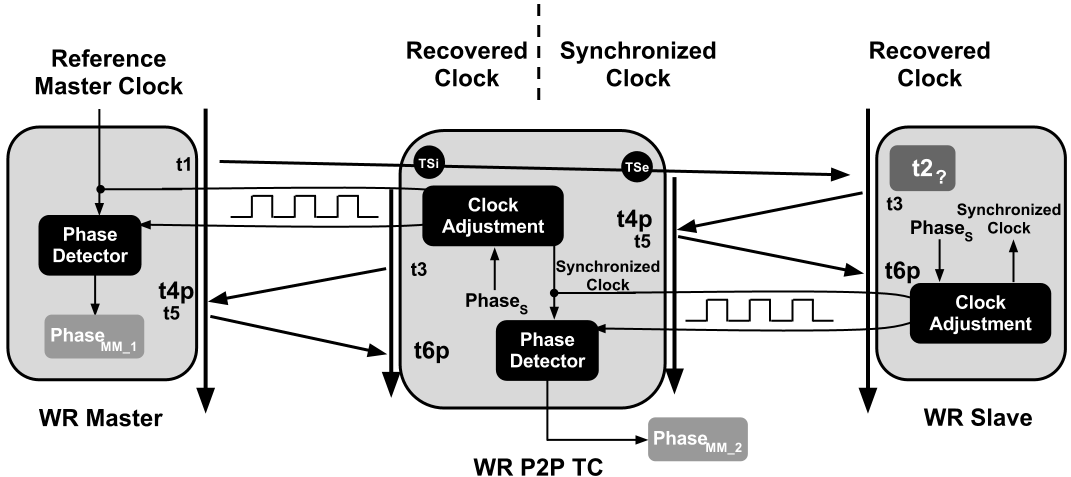
\includegraphics[scale=0.43]{fig/time_stamps_tc.png}
\caption{WR synchronization and P2P TC}
\label{fig:time_stamp}
\end{figure*}

\subsection{Maximum Update Rate}

QoS queuing

\subsection{Stability and Continuity of the Synchronization}

P2P

\subsection{WR Hardware and Software TC}

Currently the WR Switch V3 ~\cite{biblio:wrswitch} behaves as Boundary clock.
After an exhaustive examination of the WR project, the following features should be 
added to the existing gateware and software (no modifications in the hardware)
for a proof of concept WR TC implementation:

\begin{itemize}
    \item Peer Delay Mechanism 
    \item WR TC clock behaviour   
    \item Hardware process of Sync and Follow Up messages
    \item Enhanced Timestamping across TC using WR
\end{itemize}

The openness of the project \footnote{The WRS is licensed under \textit{CERN Open Hardware Licence}
~\cite{biblio:lic}  and is publicly available in the Open Hardware Repository.},
plus the amount of work already done, makes the implementation achievable with a
reasonable effort.


\FloatBarrier
